\documentclass[12pt,letterpaper]{beamer}
\usetheme{Copenhagen}
\usecolortheme{seahorse}
\setbeamertemplate{section in toc}{\inserttocsection}

\usepackage[utf8]{inputenc}
\usepackage{amsmath}
\usepackage{amsfonts}
\usepackage{amssymb}
\usepackage{graphicx}
\graphicspath{ {./images/} }
\usepackage{multirow}
\usepackage{hyperref}
\hypersetup{
    colorlinks=true,
    linkcolor=blue,
    filecolor=magenta,      
    urlcolor=cyan,
    pdftitle={Overleaf Example},
    pdfpagemode=FullScreen,
}
\title[Robotics I]
{ENGR 3421: ROBOTICS I}
\subtitle{Ultrasonic Distance Sensor}

\author[Zhang, Lin]
{Dr. Lin Zhang}
\institute[UCA] % (optional)
{
  Department of Physics and Astronomy\\
  University of Central Arkansas
}
\date[Robotics1 2021] % (optional)
{August 31, 2021}
\logo{
\includegraphics[height=1cm]{../images/uca_bear_logo.png}}


%End of title page configuration block
%------------------------------------------------------------

%------------------------------------------------------------
%The next block of commands puts the table of contents at the beginning of each section and highlights the current section:

\AtBeginSection[]
{
  \begin{frame}
    \frametitle{Outline}
    \tableofcontents[currentsection]
  \end{frame}
}
%------------------------------------------------------------

\begin{document}

%The next statement creates the title page.
\frame{\titlepage}

%---------------------------------------------------------
%This block of code is for the table of contents after the title page
\begin{frame}
\frametitle{Outline}
\tableofcontents
\end{frame}
%---------------------------------------------------------


\section{Sonar Sensor}

\begin{frame}{Ultrasound}
    Ultrasound is high-pitched sound waves with frequencies higher than the audible limit of human hearing.
    {\centering
        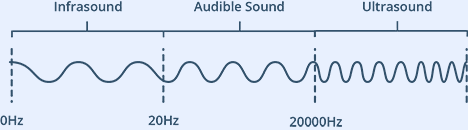
\includegraphics[width=0.8\linewidth]{ultrasound_frequency}
    }
\end{frame}

\begin{frame}{HC-SR04 Ultrasonic distance sensor}
    \begin{columns}
        \column{0.5\textwidth}
        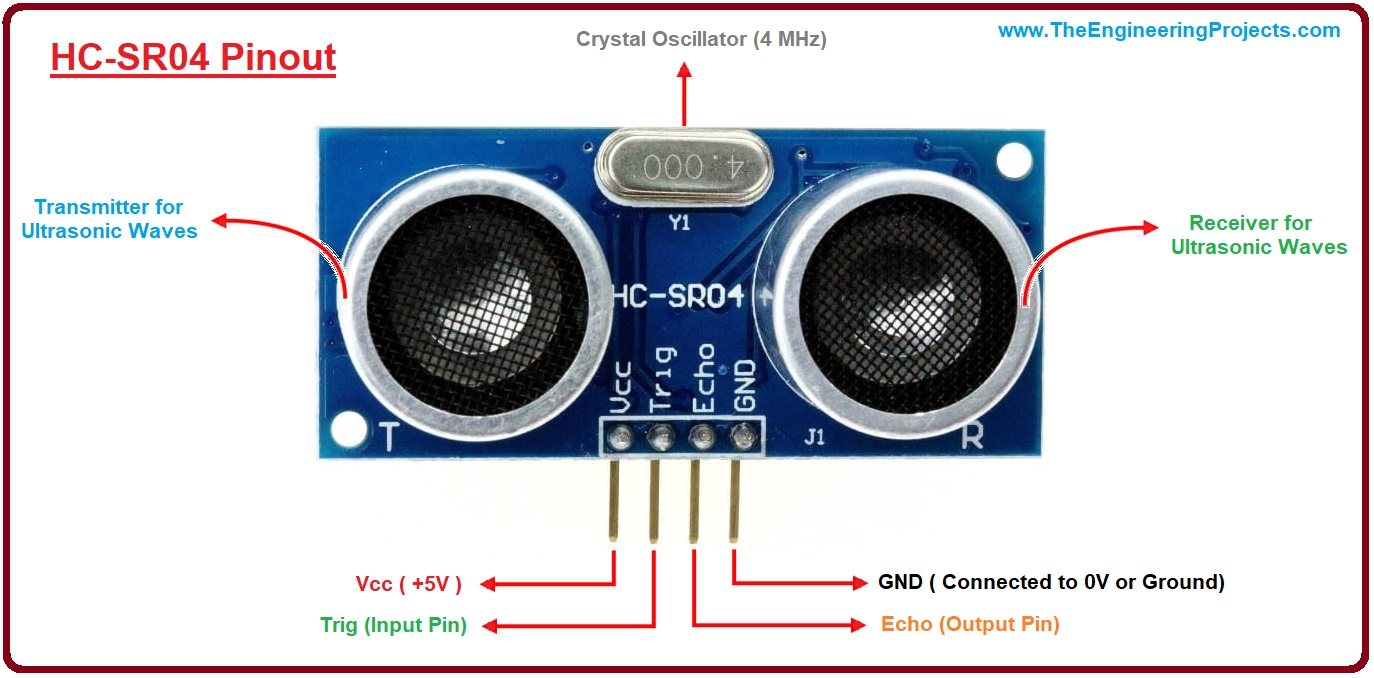
\includegraphics[width=1.1\linewidth]{HC-SR04}

        \column{0.5\textwidth}
        {\scriptsize
            \begin{itemize} 
                \item Consists of two ultrasonic transducers: a transmitter and a receiver. 
                \item The transmitter converts electrical signal into 40 KHz ultrasonic sound pulses. 
                \item The receiver listens for the transmitted pulses. 
                \item If receives the pulses back, produces an output pulse to determine the distance. 
            \end{itemize} 
        }
    \end{columns}
\end{frame}


\end{document}

